\chapter{Refining the bounds}
\label{chap:bounds}

In previous chapters we have established that $\gdist(p)$ is asymptotically logarithmic, or, more precisely, that
\begin{align}
	2.73 \approx 3 \log_3(e) < \frac{\gdist(p)}{\log(p)} < 5 \log_2(e) \approx 7.21
\end{align}
for primes \todo{$p > ?$}. The obvious question is -- what are the best possible constants in these estimates?

While the question is open, in this chapter we provide evidence which suggests that the following might be true:

\begin{conj}
\label{conj:lim-gdist}
Let $P$ be a real such that $P^3=P+1$. Then for primes $p$:
\begin{align}
	\lim_{p \rightarrow \infty} \frac{\gdist(p)}{\log(p)} = \frac{1}{\log(P)} \approx 3.56.
\end{align}
\end{conj}%

Our argument is based on the connection of $\gdist(p)$ to dissections of triangles. Let us recall that Lemma \ref{lem:gdist-leq-tn} states that $\gdist(p) \leq t(p)$ and it is conjectured that $\gdist(p) = t(p)$ (Conjecture \ref{conj:gdistp-equals-tp}).

In this chapter we present computational data of Rosendorf \cite{Rosendorf04} and of our own which support the following:

\begin{conj}
\label{conj:lim-hat-tn}
Let $P$ be a real such that $P^3=P+1$. Then
\begin{align}
	\lim_{n \rightarrow \infty} \frac{\hat t(n)}{\log(n)} = \frac{1}{\log(P)}.
\end{align}
\end{conj}%

Note that Conjectures \ref{conj:lim-hat-tn} and \ref{conj:gdistp-equals-tp} imply Conjecture \ref{conj:lim-gdist}.

In some sense, as we will see, it is easier to approach Conjecture \ref{conj:lim-hat-tn}. One of the reasons is that we do not have to restrict ourselves only to primes, but can regard all numbers equally.

%%%
%%%
%%%
\section{Padovan sequence}

\begin{defn}
\emph{Padovan sequence} is a linear recurring sequence $(a_k)_{k \geq 1}$ defined by
\cosyalign{
	a_1 = a_2 = a_3 = 1, \quad a_{k+3} = a_{k+1}+a_k \ \ \mbox{ for } n \geq 1.
}%
The first few terms are $1, 1, 1, 2, 2, 3, 4, 5, 7, 9, 12, 16,\dots$
\end{defn}

For more information about the sequence see e.g. \cite{OEIS}.

Let $P, \lambda_1, \lambda_2$ be roots of the polynomial $x^3-x-1$, where $P$ is the only real root. Then we can write explicitly
\cosyalign{
	a_k = c_0P^k + c_1\lambda_1^k + c_2 \lambda_2^k
}%
for some complex constants $c_0,c_1,c_2$. Computing the values, we get $|\lambda_1|, |\lambda_2| < 1$ and $c_0 \approx 0.545$ is a real. Therefore $a_k \sim c_0P^k$, or $\log_P(a_k) \sim k$.

The number $P \approx 1.325$ is called \emph{plastic constant}. As a side note, along with its mathematical properties, it has also its application in architecture \cite{Stewart96}.

\begin{defn}
Let $n$ be a positive integer. By $\spb(n)$ we denote an integer such that
\cosyalign{
	a_{\spb(n)-1} < n \leq a_{\spb(n)}.
}
\end{defn}

Note that $a_{\spb(n)}$ is the nearest term in Padovan sequence which is larger or equals to $n$. Also $\spb(n) \sim \log_P(n)$.

Consider a trapezoid consisting of three unit triangles. In each step, we can attach a triangle to the longest side of the shape to get a pentagon. This way we get a spiral-like tiling. By adding two more triangles to the pentagon we obtain a $\circledast$-free dissection of a triangle. (Figures \ref{fig:spiral}, \ref{fig:spiral2}.)

\begin{figure}[htb]
\centering
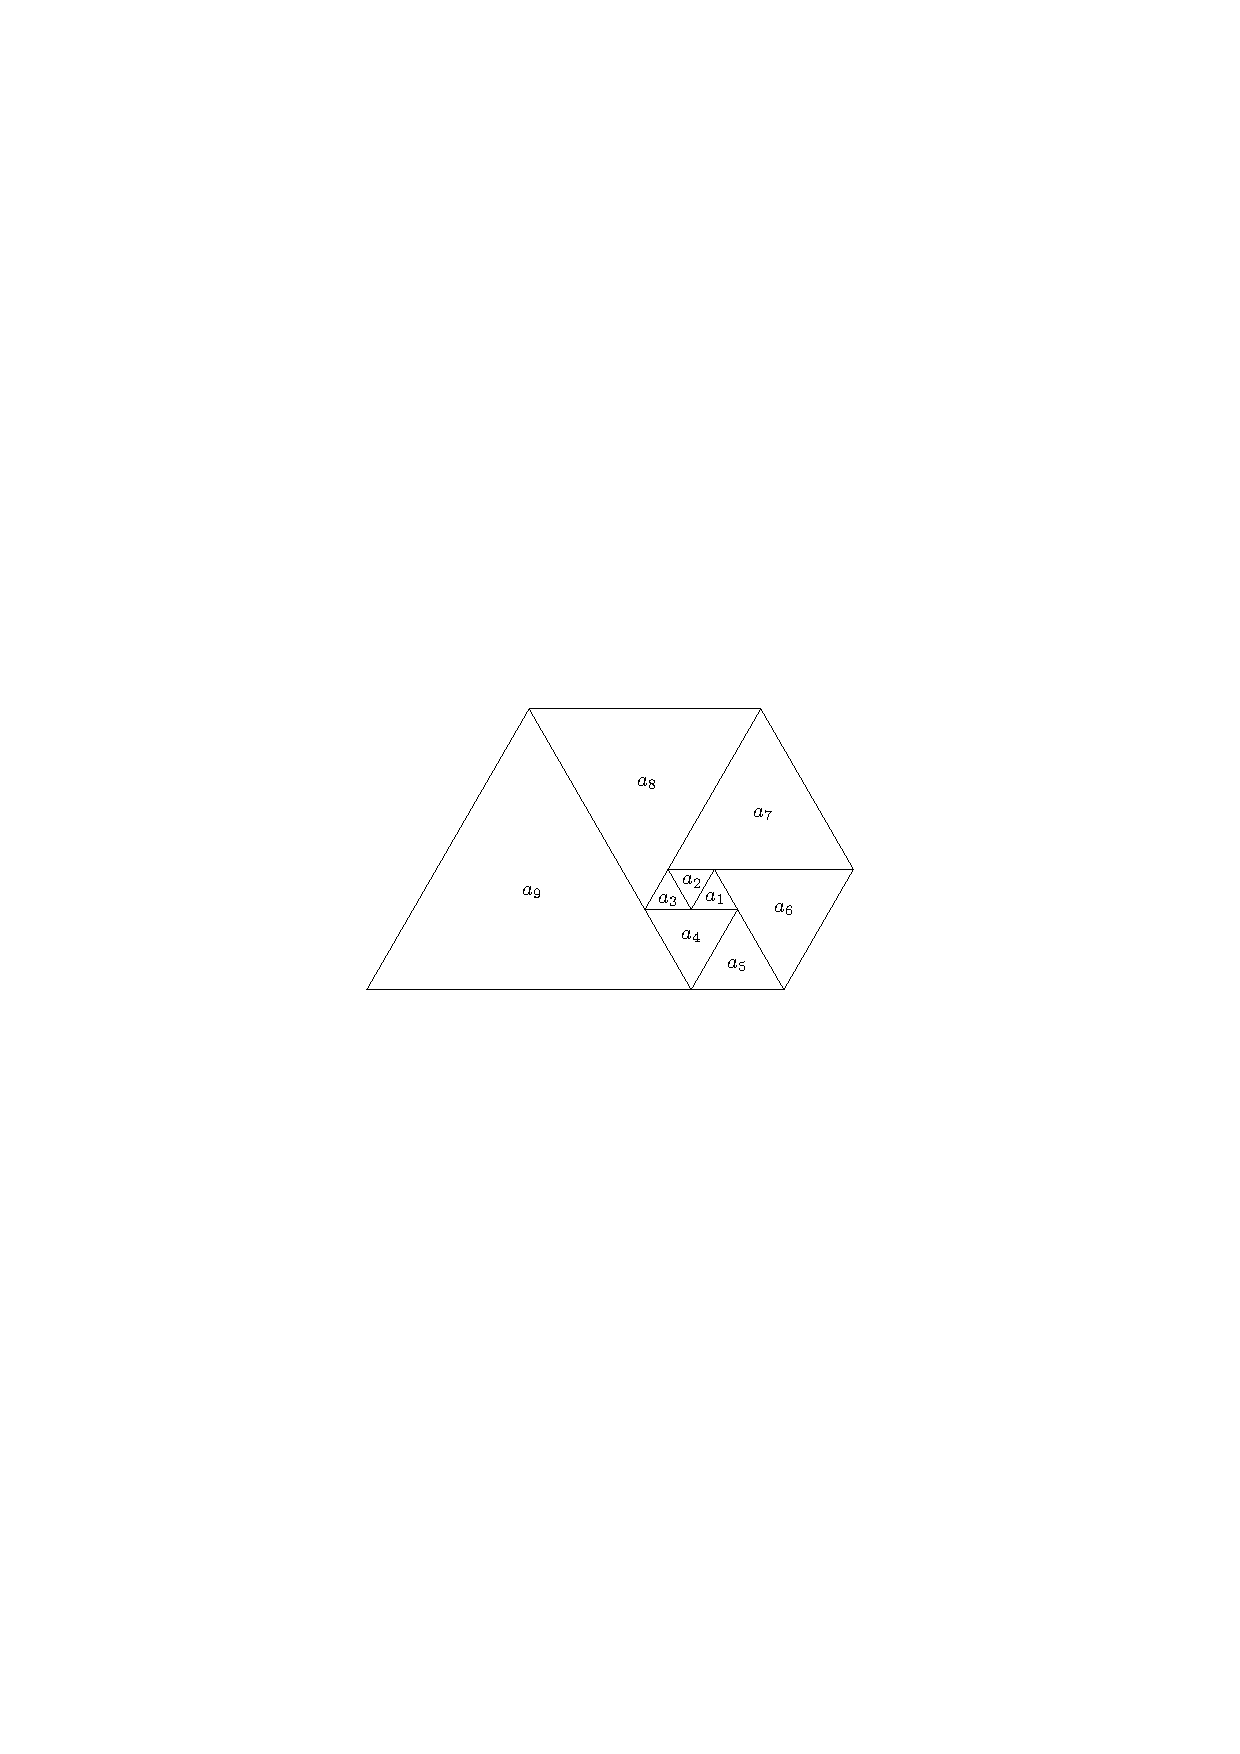
\includegraphics[width=0.6\textwidth]{img/spiral.pdf}
\caption{Spiral tiling.}
\label{fig:spiral}
\end{figure}

\begin{figure}[htb]
\centering
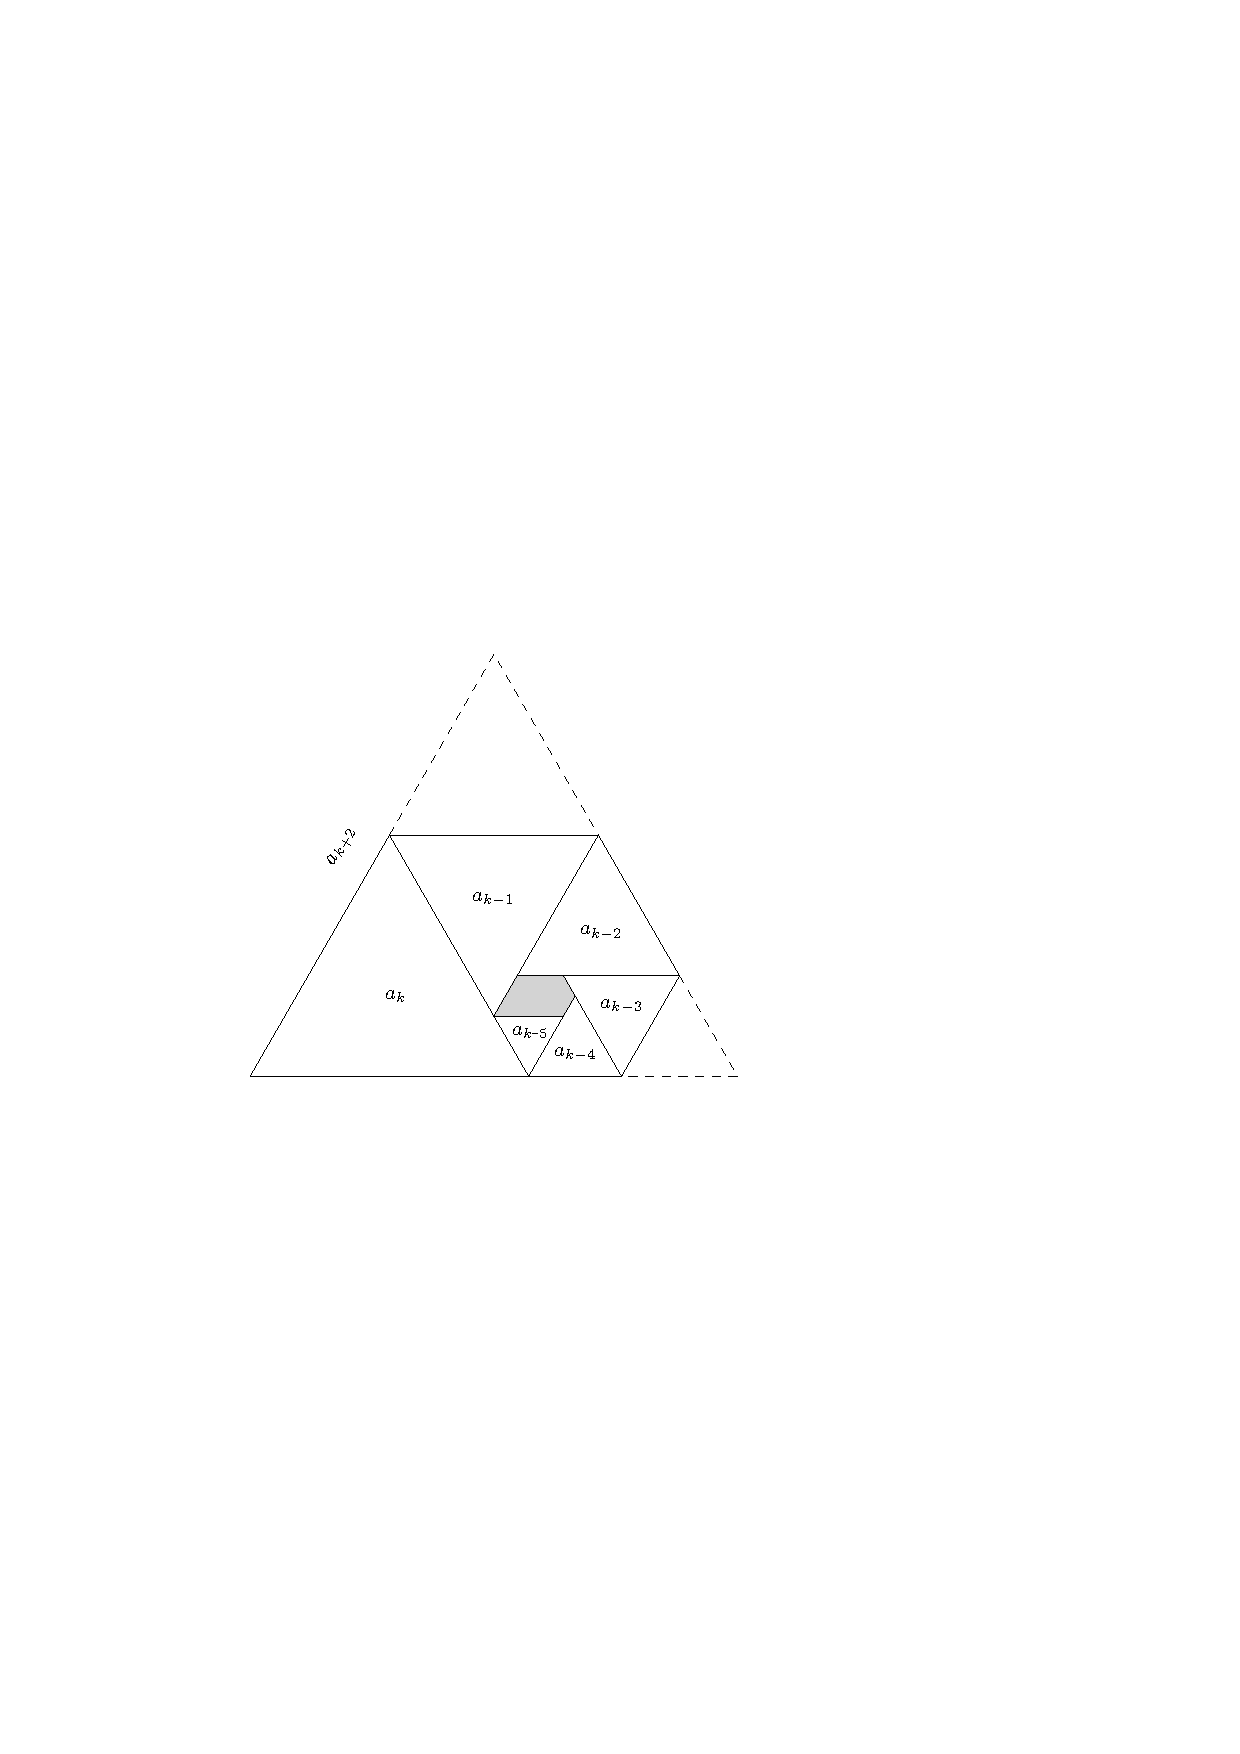
\includegraphics[width=0.6\textwidth]{img/spiral_triangle.pdf}
\caption{Completion of a pentagon into a triangle.}
\label{fig:spiral2}
\end{figure}

It is easy to derive that the sizes of the triangles are exactly the terms of Padovan sequence. Therefore we can construct a dissection of a triangle of side $a_{k+2}$ into $k+2$ triangles. Since in such a dissection there is always a triangle of side 1, we obtain
\cosyalign{
	\hat t(a_k) \leq k = \spb{a_k} \sim \log_P(a_k).
}%


%%%
%%%
%%%
\section{Rosendorf}
Based on Drápal's suggestion, Rosendorf studied in his master's thesis \cite{Rosendorf04} a modification of the spiral tiling, which can be applied to triangles of any size. Consider the following algorithm:

\begin{alg} \ 
	\begin{cosyitemize}
		\item In the beginning, from two corners of the original triangle cut off two triangles to get a pentagon or a parallelogram;
		\item Then, until the remaining shape is a triangle, cut off a triangle from the current shape to get either a pentagon, a parallelogram, a trapezoid or a triangle.
	\end{cosyitemize}
\end{alg}%

The algorithm is nondeterministic -- if the current shape is not a pentagon, we can choose the placement and the size of the triangle to be cut off. Rosendorf proved that these dissections are exactly those which are $\circledast$-free and do not contain a subset of triangles forming a proper convex hexagon. Following his notation, let us denote such a dissection as \emph{(M6)}, standing for "missing hexagon".

Rosendorf enumerated all minimal (M6) dissections of triangles of side less than 10252. The data shows that
\begin{align}
	\hat{t}(n) \leq \spb(n)+2 \qquad\hbox{for $n < 10252$.}
\end{align}

On the other hand, he also proved that at least $\spb(p)$ triangles are needed in an (M6) dissection of a triangle of prime side $p$. That, however, is not true when we allow all $\circledast$-free dissections.


%%%
%%%
%%%
\section{Enumerations of minimal dissections}

To support Conjecture \ref{conj:lim-hat-tn}, we generated all triangle dissections up to size 23 and therefore established values of $t(n)$ and $\hat t(n)$ for $n \leq 416$. For comparison, in \cite{DrapalHamalainen10} Drápal and Hämäläinen were able to generate dissections up to size 20, which corresponds to $n \leq 160$. They were, however, primarily interested in the number of triangulations of given size and perfect dissections (no two triangles of the same orientation have the same size), not in the values of $t(n)$ and $\hat t(n)$.

We use essentially the same algorithm as in \cite{DrapalHamalainen10}.\footnote{Although it is not absolutely clear from their paper, our implementation has probably better time complexity.} As we have shown, from a triangle dissection it is possible to construct a latin bitrade, and thus also a graph of the bitrade. All such graphs can be effectively generated by plantri software \cite{BrinkmannMcKay99}. Our algorithm computes all triangle dissections which correspond to a given graph.

\todo{@ Potrbujem najprv odseparovat??}

\begin{lem}
Let $D$ be a dissection of $\Delta_n$ and $(T^*, T^\vartriangle)$ the corresponding bitrade. Then
\cosyalign{
	@M_{T^*}x^T = (n,0,\dots,0)^T
}%
has the only solution $(x_1,\dots,x_?,\dots)$.
\end{lem}
\begin{proof}
@ Spherical ... dimension ... full rank. \\
@ The solution is solution
\end{proof}

\begin{lem}
Let $D$ be a prime dissection of $\Delta_n$ and $(T^*, T^\vartriangle)$ the corresponding bitrade. Then
\cosyalign{
	@M_{T^*}x^T = (1,0,\dots,0)^T
}%
has the only solution in which $n = \lcm(blah)$.
\end{lem}
\begin{proof}
@ proof
\end{proof}

\begin{cor}
The vector $x$ is $k$-th column of $M_T^{-1}$.
\end{cor}%

The algorithm to generate all triangle dissections is as follows:

\begin{alg}\ 
\begin{cosyenumerate}
	\item Use plantri to generate planar Eulerian triangulation.
	\item Construct corresponding separated bitrade $(T,T')$.
	\item Find $M_T^{-1}$. Every \todo{row} describes a homotopy of $T$ into $\Z\times\Z\times\Z$.
	\item Check that the homotopy is embedding. Then it must correspond to a triangle dissection.
	\item Repeat for $T'$.
\end{cosyenumerate}
\end{alg}%

The generated values of $\hat t(n)$ are listed in \todo{Table}. Because we generated all dissections up to size $23$, we also know that $\hat t(n) = 24$ for those $n$, for which we know at least one dissection into $24$ triangles. The values suggestively keep close to $\spb(n)$. We conjecture the following:

\begin{conj} $\spb(n)-1 \leq \hat t(n) \leq \spb(n)$.
\end{conj}%

Conjencture \ref{conj:lim-hat-tn} then follows by $\spb(n) \sim \log_P(n) = \log(n)/\log(P)$.



